
%(BEGIN_QUESTION)
% Copyright 2008, Tony R. Kuphaldt, released under the Creative Commons Attribution License (v 1.0)
% This means you may do almost anything with this work of mine, so long as you give me proper credit

Something is wrong with this building security alarm system circuit.  The alarm siren energizes even when all the windows and doors are shut.  The only way to silence the alarm is to use the ``override'' key switch:

$$\includegraphics[width=15.5cm]{i03195x01.eps}$$

Using your logic probe, you measure a high signal at TP7 and a low signal at TP6 with all windows and doors shut, and with the key switch in the ``override'' position.  From this information, identify two possible faults (either one of which could account for the problem and all measured values in this circuit).  Then, choose one of those possible faults and explain why you think it could be to blame.  The circuit elements you identify as possibly faulted can be wires, traces, and connections as well as components.  Be as specific as you can in your answers, identifying both the circuit element and the type of fault.

\medskip
\goodbreak
\item{} Circuit elements that are possibly faulted
\item{1.}
\item{2.} 
\end{itemize}

\medskip
\goodbreak
\item{} Explanation of {\it why} you think one of the above possibilities could be to blame

\vfil 

\underbar{file i03195}
\eject
%(END_QUESTION)





%(BEGIN_ANSWER)

This is a graded question -- no answers or hints given!

%(END_ANSWER)





%(BEGIN_NOTES)

With all doors and windows shut, both OR gates $U_1$ and $U_2$ should be receiving low signals, resulting in low signals sent to the OR gate $U_3$, resulting in a low signal at TP7.  A high signal at TP7 will sound the alarm provided the key switch is in the ``Normal'' position.  So, the fact we have a high signal at TP7 with all windows and doors shut tells us the problem lies with $U_3$ or to the left of it.

\vskip 10pt

Note: the following answers are not exhaustive.  There may be more circuit elements possibly at fault!

\begin{itemize}
\item{} Circuit elements that are possibly faulted
\item{1.} $SW_1$ contacts not closing (dirty or worn)
\item{2.} $SW_2$ contacts not closing (dirty or worn)
\item{3.} Broken wire between $SW_1$ and TP1
\item{4.} Broken wire between $SW_2$ and TP2
\item{5.} Broken wire between $SW_1$ and ground
\item{6.} Broken wire between $SW_2$ and ground
\item{7.} $U_3$ output failed high
\item{8.} $U_1$ output failed high
\end{itemize}

%INDEX% Troubleshooting review: electric circuits

%(END_NOTES)


